\subsection{Validierung}
\begin{frame}{Validierung}
	\textbf{k-fache Kreuzvalidierung}
	\begin{itemize}
		\item beachtet Abhängigkeit der Datenpunkte nicht
		\item zerstört zeitliche Komponente
		\item verwendet eventuell zukünftige Beobachtungen für Prognose der Gegenwart
	\end{itemize}
	$\Rightarrow$ \textbf{Kreuzvalidierung für Zeitreihen}
\end{frame}

\begin{frame}{Validierung}
	\begin{figure}[h]
		\centering
		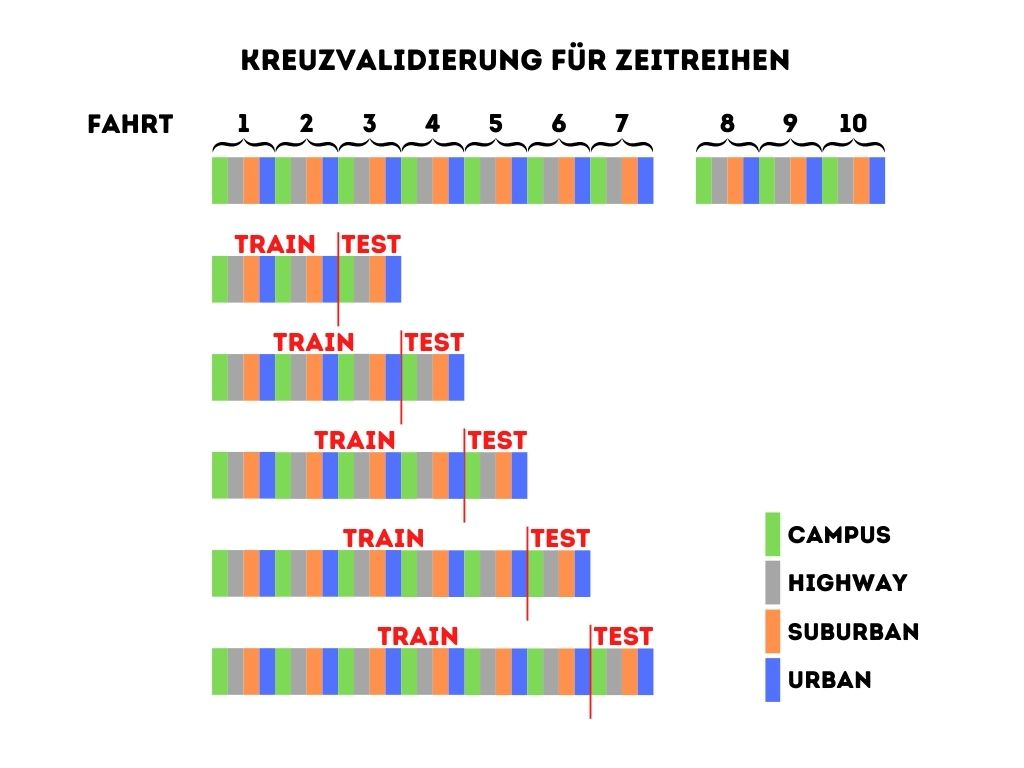
\includegraphics[scale=0.33]{kreuzvalidierung}
		\caption{Einteilungen in Trainings- und Testdatensätze bei der Kreuzvalidierung für Zeitreihen.}
		\label{kreuzvalidierung}
	\end{figure}
\end{frame}
